\documentclass[letterpaper,oneside,12pt]{article}
%\documentclass[letterpaper,oneside,12pt]{report}
\usepackage{graphicx}
\usepackage{rotating}
\usepackage[american]{babel}

\selectlanguage{american}

% page layout
%  \setlength{\hoffset}{-1in} 
  %\setlength{\voffset}{-1in}
%  \setlength{\textwidth}{15cm}
%  \setlength{\oddsidemargin}{3.5cm}
%  \setlength{\evensidemargin}{0.2cm}
%  %\setlength{\topmargin}{2.5cm}
%  \setlength{\headsep}{5ex}
%  \setlength{\textheight}{22cm}
%  \renewcommand{\baselinestretch}{1.05}
%  \raggedbottom
%  \newlength{\pictheight}
%  \setlength{\pictheight}{\textheight}
%  \addtolength{\pictheight}{-2cm}

% document
\begin{document}

%\begin{titlepage}
\hspace{-7mm}
\begin{minipage}{\textwidth}
\begin{center}
\vspace{.5cm}
{\huge \bf Software Design Document\\[1.5ex]}
{\large \bf for a specific implementation of `BCI2000'}
\\[1.5cm]
{\Large Gerwin Schalk\\}
{\Large Thilo Hinterberger\\}
{\Large Dennis J. McFarland\\[1.5cm]}
%
\begin{minipage}{13cm}
  \begin{minipage}[c]{13cm}
    \begin{center}
      {\Large \bf New York State Department of Health\\[2ex]}
      {\large \bf Wadsworth Center\\[0.5ex]
       Laboratory of Nervous Systems Disorders\\[4ex]}
      {\Large \bf Eberhard--Karls--Universit\"at T\"ubingen\\[2ex]}
      {\large \bf Medizinische Fakult\"at\\[0.5ex]
       Institut f\"ur Medizinische Psychologie\\[0.5ex]}
    \end{center}
  \end{minipage}
  \\[1.0cm]
  \begin{minipage}[c]{6cm}
    \centerline{
\includegraphics{figures/DOHlogo}}
  \end{minipage}
  \hspace{1.5cm}
  \begin{minipage}[c]{3cm}
    \centerline{
\includegraphics{figures/EKUlogo}}
  \end{minipage}
\end{minipage}
%
\\[0.5cm]
\textbf{Sponsors} \\
\textit{Jonathan R. Wolpaw and Niels Birbaumer}
\\[1.0cm]
{Albany, NY} \\[1ex]
{February 2000--May 2001}
\\[1ex]Updated May 2003, J\"urgen Mellinger
\end{center}
\end{minipage}
\end{titlepage}

\title{D3Box Task for BCI2000}
\author{Shidong Zheng, Melody Moore, Gerwin Schalk}
\maketitle

\newpage
\tableofcontents

\newpage 

\begin{abstract}

The purpose of the D3Box task is to provide a BCI2000 User Application module 
that can realize 1D, 2D, or 3D cursor movement tasks. It is intended to 
provide a superset of the functionality provided in the RJB and D2Box task. This 
task is implemented using a generic 3D API based on OpenGL that may be used to 
create other 3D user applications. 

\end{abstract}

\section{Introduction}

The D3Box task implements a cursor movement task based on a 3-dimensional 
control signal communicated to it by an appropriate BCI2000 Signal Processing 
module. This task is characterized by a sequence of five subsequent stages that 
are illustrated in Figure \ref{fig:timeline}. In stage 1, the screen shows an 
empty workspace. This period is called \emph{Inter-Trial Interval}. 
Subsequently, a target (that is represented as a cuboid) appears in one out of 
\emph{n} possible locations. This period is called \emph{Pre-Trial Pause}. After 
the pre-trial pause, the cursor appears in stage 3. It immediately starts to 
move as determined by the 3-dimensional control signal. During stage 3 and 4,
the user's task is to move the cursor towards and into the target. This period
of cursor movement is called the \emph{Feedback Period} or \emph{Trial Period}.
Period 4 can end in one of three ways: Either the cursor hits the correct target, 
it misses by hitting any other of the defined targets, or the feedback period takes
too long and times out. Stage 5, the \emph{Reward Period}, follows stage 4.
The cursor disappears and the target changes its color to indicate completion
of the trial period. After a defined duration, the target disappears and the
next trial starts with an Inter-Trial Interval.

\begin{figure}[ht]
 \centerline{\scalebox{0.55}{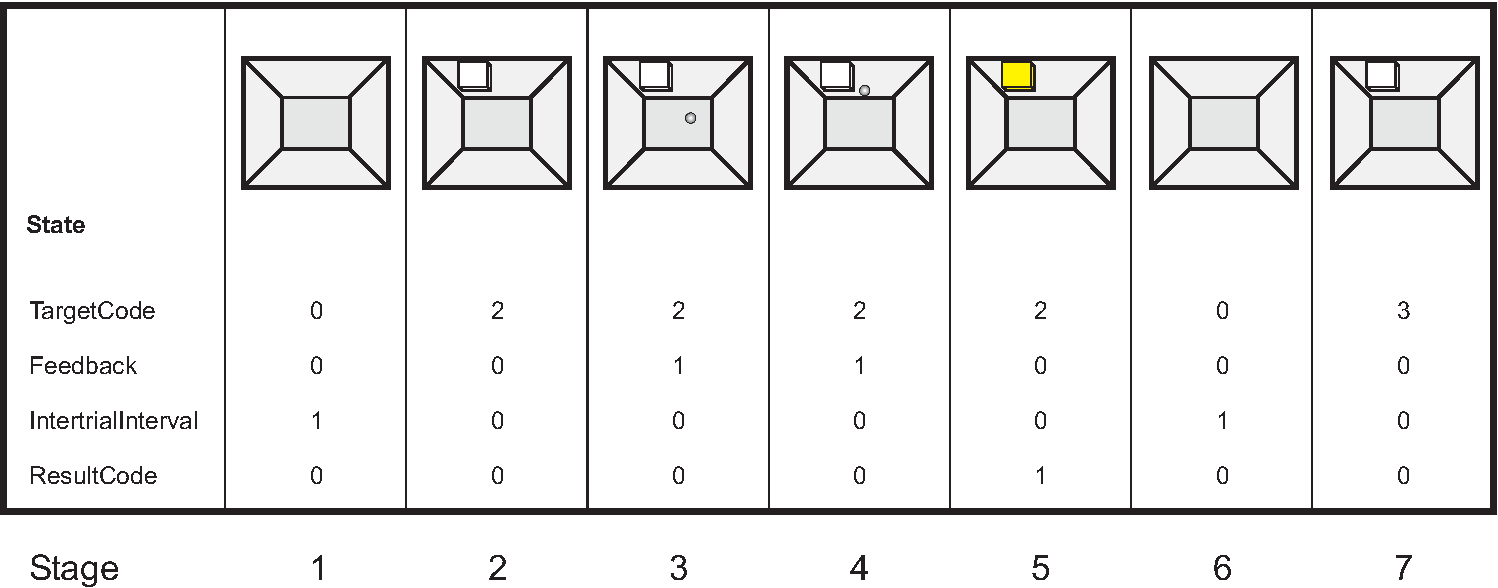
\includegraphics{figure/timeline.pdf}}}
 \caption{The time line of the D3Box task. The BCI2000 state variables
          that encode the trial sequence are \emph{TargetCode} (i.e., which
          of the defined targets is currently present on the screen),
          \emph{Feedback} (i.e., whether or not user feedback
          is provided by the cursor), \emph{IntertrialInterval} 
          (i.e., whether or not we are presently in this period), 
          and \emph{ResultCode} (i.e., which of the defined targets 
          has been selected).}
 \label{fig:timeline}
\end{figure}

\section{Visual Representation}

The visual representation of the D3Box task is represented in Figure 
\ref{fig:d3boxscreen}. It consists of a 3-dimensional workspace that can (if 
selected) be indicated by five bounding rectangles. These rectangles can have a 
user-selectable texture, which is the same for each rectangle. Targets are 
represented by cuboids, whose edges can also have a particular texture. 
Finally, the cursor is represented by a sphere. It also may have a user-defined 
texture. To facilitate depth perception, the cursor's color provides an 
additional cue about the cursor's Z position as follows. The operator specifies 
two colors that indicate the cursor's color at Z position +32767 and -32767. In 
other words, a cursor at position +32767 or -32767 will have the corresponding 
color. For any color between these extremes, the cursor's color will be linearly 
interpolated between the two colors. (Specifically, each of the three color 
components (i.e., red, green, and blue) will be interpolated to result in the 
cursor's color for a given Z position.)

\begin{figure}[ht]
 \centerline{\scalebox{0.55}{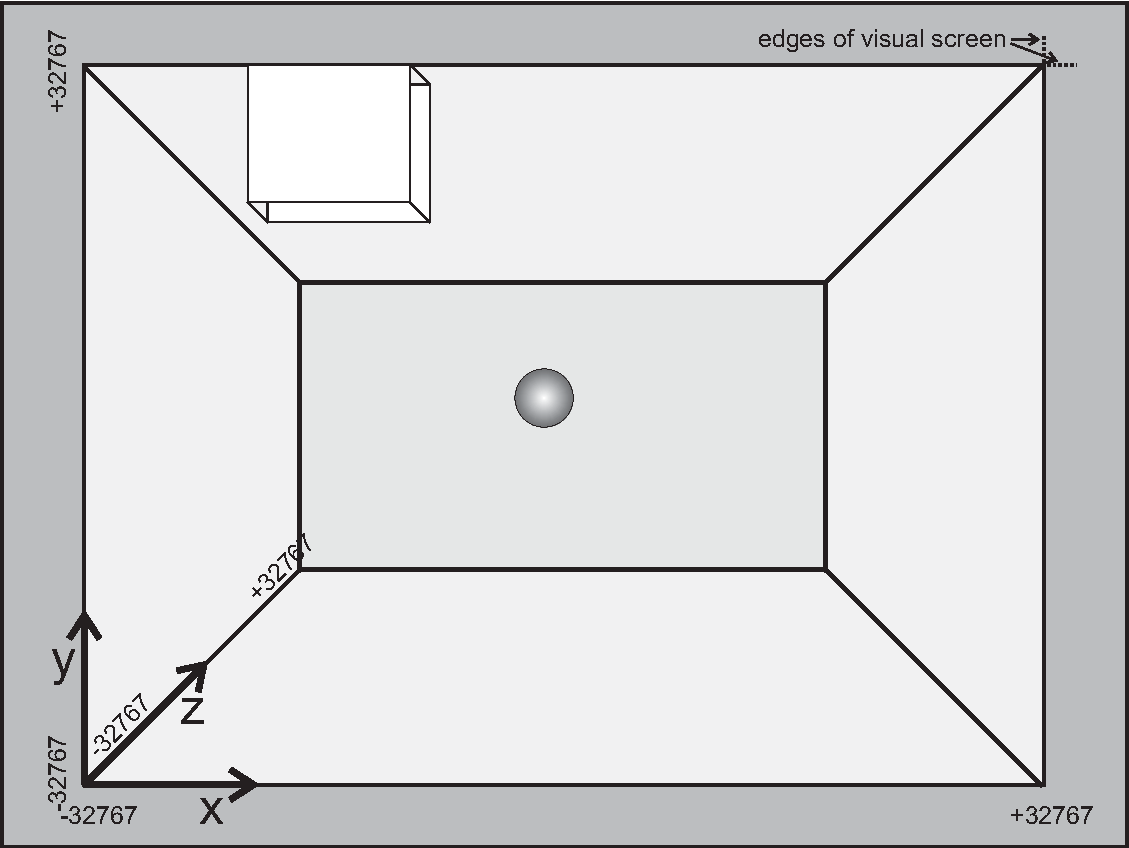
\includegraphics{figure/d3boxscreen.pdf}}}
 \caption{The screen layout of the D3Box task.}
 \label{fig:d3boxscreen}
\end{figure}


\section{Control of the D3Box Task}

The cursor in the D3Box task can be controlled in two different ways. The first 
option is to control the cursor using the control signals communicated to it 
from an appropriate BCI2000 Signal Processing module. The second option is to 
control the cursor using a standard joystick that is attached to the computer. 
In this case, joystick movements left/right and up/down control the 
cursor's x and y position, respectively. If the user presses the joystick 
button, the cursor slowly moves towards the front of the workspace (i.e., 
towards the screen). If the user does not press the joystick button, the cursor 
slowly moves towards the back of the workspace (i.e., away from the screen). 
Whether the cursor is controlled by the joystick or by the control signals 
coming from the signal processing module is defined by a parameter.

\section{Parameters}
This section describes the parameters that configure the D3Box task.
The parameters are grouped by the section they belong to, i.e., the
tab in the Operator's config menu they appear in.

\flushleft{Section \emph{Joystick}:}
\begin{itemize}
  \item {\tt JoyXGain} After subtracting XOffset, the joystick signal
        in X is multiplied with JoyXGain. Thus, if JoyXGain is higher,
        horizontal cursor movement will be more reactive to joystick
        movement.
  \item {\tt JoyYGain} Same as JoyXGain, but for Y dimension.
  \item {\tt JoyZGain} Same as JoyXGain, but for Z dimension.
  \item {\tt UseJoyStick} If this parameter is 0, the cursor is controlled
        by the three control signals communicated to the D3Box task by
        Signal Processing. If it's set to 1, the cursor is controlled by the joystick.
  \item {\tt XOffset} This value is subtracted from the current
        joystick X direction. This can be used to either compensate for
        or to create a bias in the joystick movement.
  \item {\tt YOffset} Same as XOffset, but for Y dimension.
  \item {\tt ZOffset} Same as XOffset, but for Z dimension.
\end{itemize}

\flushleft{Section \emph{Targets}:}
\begin{itemize}
  \item {\tt IncludeAllTargets} If 1, the trial will end if the cursor hits
        any of the specified targets, even though only one target is on
        the screen at a given time. If 0, the trial will end only if the cursor
        hits the visible target or if the trial times out.
  \item {\tt NumberTargets} Specifies the number of targets. This has to correspond
        to the number of columns in the TargetPos matrix.       
  \item {\tt StartCursorX} Starting X coordinate of the cursor (in percent of screen width).
  \item {\tt StartCursorY} Starting Y coordinate of the cursor (in percent of screen height).
  \item {\tt StartCursorZ} Starting Z coordinate of the cursor (in percent of screen depth).
  \item {\tt TargetPos} This is a matrix that defines the targets and their
        positions on the screen. Each target occupies one column and 10 rows.
        In ascending order starting with one, the rows correspond to:
        X coordinate of midpoint of target, Y coordinate of midpoint of target,
        Z coordinate of midpoint of target, width of target, height of target,
        depth of target, X adaptation coordinate, Y adaptation coordinate, Z adaptation
        coordinate, adaptation code. The first six rows define the position and
        spatial extent of each target in screen coordinates, i.e., they are defined 
        in percent of screen width, height, or depth. For rows 7-10, the
        adaptation coordinates and adaptation code, the values in these
        rows are assigned to states XAdapt, YAdapt, ZAdapt, AdaptCode, 
        respectively for the target that is currently visible on the screen.
\end{itemize}

\flushleft{Section \emph{UsrTask}:}
\begin{itemize}
  \item {\tt BorderTexture} If defined, this defines the full path to the 
        texture that is applied to the rectangles that enclose the workspace.
        The texture has to be in BMP format.
        If this parameter is not defined (i.e., the screen is empty), no
        texture is applied. The D3Box task sends a BCI2000 warning message if
        the texture is not found.
  \item {\tt CursorSize} Defines the size of the cursor in percent of screen width.
  \item {\tt CursorTexture} Defines the full path to the texture that is applied
        to the cursor. See {\tt BorderTexture}.
  \item {\tt CursorColorFront} Color of cursor if cursor is at the very front
        of the workspace (i.e., Z of -32767) in RGB\footnote{For convenience, 
        RGB values may be entered in hexadecimal notation, e.g. 
        \texttt{0xff0000} for red.}
  \item {\tt CursorColorBack} Color of cursor if cursor is at the very back
        of the workspace (i.e., Z of +32767) in RGB. Cursor color between these
        extremes is linearly interpolated.
  \item {\tt FeedbackDuration} This parameter defines the maximum trial duration
        in feedback updates\footnote{A feedback update is defined as the ratio
        of $\frac{SampleBlockSize}{Samplingrate}$ in seconds. Thus, for a blocksize
        of 16 and a sampling rate of 160 Hz, this comes out to 0.1 seconds=100 ms.
        In this example, if {\tt FeedbackDuration} were specified as 80, the trial
        would time out after 8 seconds.}.
  \item {\tt ItiDuration} The duration of the \emph{Inter Trial Interval}, i.e.,
        the time that the empty workspace is shown without a target or a cursor.
        This time is defined in feedback updates.
  \item {\tt PreTrialPause} The duration of the \emph{Pre-Trial Pause}, i.e.,
        the time the target is visible but the cursor is not.
        This time is defined in feedback updates.
  \item {\tt RewardDuration} The duration of the \emph{Reward Period}, i.e.,
        the time the target flashes after it is hit by the cursor.
  \item {\tt TargetTexture} Defines the full path to the texture that is applied to 
        each target.
  \item {\tt TimeLimit} Defines the maximum time of the session in seconds. The D3Box
        task will automatically suspend if a trial completes and the session has been
        running for the defined period.
  \item {\tt WinHeight} Width of the D3Box task's window in pixels.
  \item {\tt WinWidth} Height of the D3Box task's window in pixels. 
  \item {\tt WinXpos} Top Edge of the D3Box task's window in pixels.
  \item {\tt WinYPos} Left Edge of the D3Box task's window in pixels. 
\end{itemize}

\section{States}

The time line of stimulus delivery is encoded in state variables as defined in
Table~\ref{tab:states}.
\begin{table}
\begin{center}
\begin{tabular}[ht]{|l|l|l|}
\hline
\bf{State Name}& \bf{Bits}            & \bf{Description} \\
\hline
\hline
 TargetCode & 8 & target ID of the currently active target, \\
            &   & or 0 if no target is on the screen \\
 ResultCode & 8 & target ID of the currently selected target, \\
            &   & or 0 if no target selected \\
 IntertrialInterval & 1 & 1 if we are in the Inter-Trial Interval \\
            &   & or 0 otherwise \\
 Feedback   & 1 & 1 if the cursor is visible on the screen \\
            &   & or 0 otherwise \\
 CursorPosX & 16 & X position of the cursor if cursor present, \\
            &   & or 0 is the cursor is not visible \\
 CursorPosY & 16 & Same as CursorPosX but for Y coordinate \\
 CursorPosZ & 16 & Same as CursorPosX but for Z coordinate \\
 XAdapt     & 16 & XAdapt value of target as defined by TargetPos \\
            &    & matrix, or 0 if target is not visible \\
 YAdapt     & 16 & Same as XAdapt, except for Y dimension \\
 ZAdapt     & 16 & Same as XAdapt, except for Z dimension \\
 AdaptCode  & 16 & AdaptCode value of target as defined by TargetPos \\
            &    & matrix, or 0 if target is not visible \\
 StimulusTime & 16 & Time of feedback (i.e., cursor movement) update in ms \\
\hline
\end{tabular}
\caption{Encoding scheme for this task.}
\label{tab:states}
\end{center}
\end{table}

\newpage
\section{The 3D API}

\subsection{Introduction}

The D3Box task is based on the 3D API created by Shidong Zheng. The API
is located in the Application/shared/3DAPI directory. Figure \ref{fig:environment}
and the following sections describe its capabilities.


\begin{figure}[ht]
 \centerline{\scalebox{1}{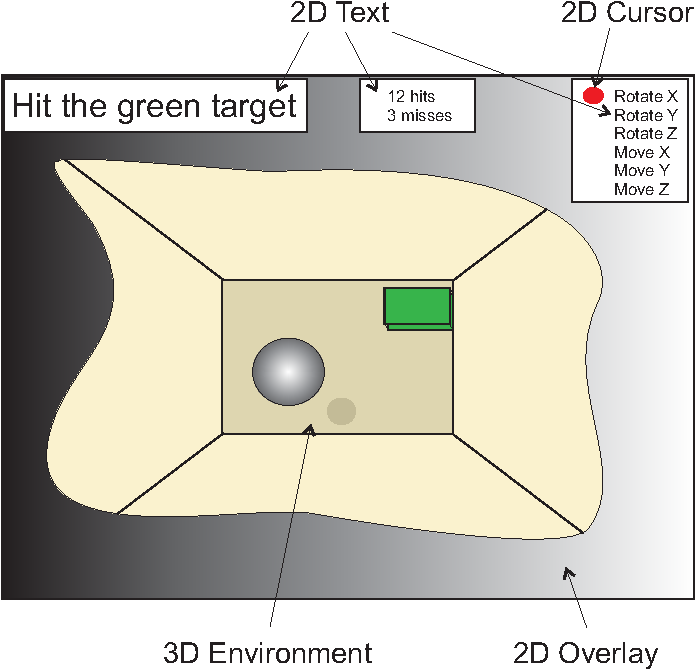
\includegraphics{figure/environment.pdf}}}
 \caption{Graphical Environment.}
 \label{fig:environment}
\end{figure}

\subsection{Rendering}



\subsection{The 3D Environment}

\subsubsection{Predefined Graphic Primitives}
The 3D environment supports any number of predefined graphic primitives. 
Each graphic primitive can be assigned a number of different properties. 
These are:
\begin{itemize}
 \item Element ID
 \item Primitive ID
 \item Primitive-specific properties
 \item Generic properties
       \begin{itemize}
        \item Brightness (0-255)
        \item Transparency (0-255)
        \item Color (RGB)
        \item Texture
       \end{itemize}
\end{itemize}
Supported primitives are spheres (i.e., primitive ID 1), cuboids (i.e., primitive ID 2), 
and infinite planes (i.e., primitive ID 3). The position
of a sphere is defined by midpoint (XYZ) and radius. Textures are mapped using
circular mapping using arbitrary alignment. The position of a cuboid is defined
by a midpoint (XYZ) and a width, height, and depth (to define the extend in 
X, Y, and Z, respectively). Texture mapping is defined by the orientation and
size of a texture. The only supported mapping type is parallel mapping.
Infinite planes are defined by three points in XYZ coordinates. The only supported
texture mapping type is parallel mapping with the texture being parallel to the plane.

Once created, there are certain functions that can be applied to any element.
\begin{itemize}
 \item Change properties
 \item Turn on/off
 \item Move midpoint to XYZ
 \item Test for collision with another element
 \item Rotate element with rotation defined by
       \begin{itemize}
        \item Angles in X, Y, Z
        \item Reference point in X, Y, Z
       \end{itemize}
\end{itemize}


\subsubsection{Custom Graphic Primitives}

In addition to built-in primitives, the system also supports custom graphic 
primitives. These primitives can be defined by loading their 3D structure from a 
file and they support the same methods as the predefined primitives except 
collision detection.


\subsubsection{3D Text}

The system supports any number of 3D text elements. Each text element
is defined by
\begin{itemize}
 \item Font
 \item Font size
 \item Caption
 \item Brightness (0-255)
 \item Transparency (0-255)
 \item Color (RGB)
 \item Origin (XYZ)
 \item Direction (XYZ)
\end{itemize}

The text elements support methods to modify their properties and to turn
them on or off.


\subsubsection{Camera}
The 3D environment supports one camera with the following properties:
\begin{itemize}
 \item Camera View Point (XYZ)
 \item Aim Point (XYZ)
 \item Focal Length
 \item Camera Orientation (what is "up" for the camera) (angle)
\end{itemize}


\subsubsection{Light Source}
The 3D environment supports one omni-directional light source. The features that 
describe this light source are:
\begin{itemize}
 \item Position (XYZ)
 \item Brightness (0-255)
 \item Color (RGB)
\end{itemize}
In addition, the brightness of white ambient background lighting can be defined.


\subsection{The 2D Overlay}

The 3D display can be overlayed by a 2D display (see Figure 
\ref{fig:environment}. This overlay supports a picture with alpha channel (i.e., 
transparency map), 2D text and a 2D cursor.

\subsubsection{Overlay Picture}

An overlay picture can be defined by loading it from disc. This picture is 
stretched to match the window size. Optionally, a transparency map can be 
defined (i.e., in essence, another picture) whose brightness level defines the s
transparency of the overlay. This can create an effect as shown in Figure 
\ref{fig:environment}. Once defined, an overlay image can be turned on or off.

\subsubsection{2D Text}

The system supports any number of 2D text elements. Text elements are always 
displayed on top of the overlay picture. The texts' background is transparent 
and the text itself does not destroy the overlay picture. For each 2D text 
element, the following properties can be defined:

\begin{itemize}
 \item Position (XY)
 \item Font
 \item Size
 \item Color (RGB)
\end{itemize}


\subsubsection{2D Cursor}

The system supports one 2D cursor that is always presented as a circle
that is filled with a particular color. Specifically, a 2D cursor has
the following properties:

\begin{itemize}
 \item Position (XY)
 \item Size
 \item Color (RGB)
\end{itemize}


%\appendix

\end{document}

